\section{Mise en œuvre de la solution} 

La base de données étant un élément essentiel du projet, il se devait d’être très générique. En effet, cette contrainte fait partie du cahier des charges. Elle doit pouvoir accueillir les données des capteurs déjà existant mais aussi des capteurs qui pourraient être ajouter plus tard. Cette base doit pouvoir sauvegarder aussi bien les données des capteurs que leurs caractéristiques et les métas donnés liées aux à ces derniers. 

Mais, bien que celle-ci soit très importante, il s’est avéré qu’il serait plus judicieux de ne pas tout de suite se mettre à le modéliser, mais plutôt de commencer par la partie extracto-chargeur des données météo. Tout cette notion aux tours des capteurs ne m’était pas familier, il aurait été bien plus difficile pour moi de le modéliser sans avoir pu manipuler certaines de ses données capteurs. Avec mon maître de stage on est parti sur un petit schéma tout simple, facile à comprendre, pour avoir une idée générale et on s’est réservé le droit de le modifier et de l’améliorer tant que cela soit possible. 

Pendant ce temps, j’ai pu commencer à travailler sur le petit programme extracto-chargeur de données météo des stations se trouvant sur le site de Montoldre. Ainsi j’ai pu appréhender la notion de données sur les données en générale et les données météo en particuliers.  

 

\subsection{Programme extracto-chargeur de données météo}

Sur le site de Montoldre, deux stations météo avaient été installés. Valentin Mère, un autre stagiaire sur le même projet basé sur le site de Montoldre s’était occupé de la partie acquisition de données comme par exemple installer et tester le bon fonctionnement d’une station. Et moi, depuis le site d’IRSTEA Aubière, j‘avais accès aux données via le réseau Intranet net de l’IRSTEA. Une visite sur les lieux m’a permis de me rendre compte des dispositifs avec lesquelles je travaillais à distance.  

\subsection{Les Stations météo du site de Montoldre} 

\subsubsection{Station météo sencrop}

\begin{wrapfigure}{r}{.3\textwidth}
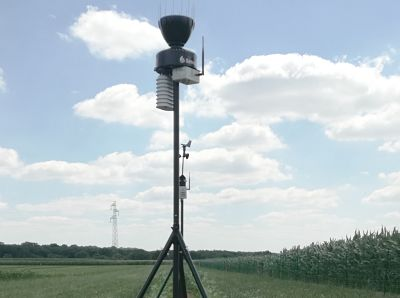
\includegraphics[width=4cm]{images/imageRang3.jpg}
\end{wrapfigure}
Sencrop est un ensemble de deux stations, un pluviomètre(raincrop) et un annémomètre(windcrop) produit par une socité française basée à Lille et spécialisé dans la météo pour l’agriculture. La station sencrop est dotée de capteurs qui enregistrent la pluviométrie, la température de l’aire, l’hygrométrie, la vitesse et la direction du vent. Elle envoie ses données toutes les quinze minutes via une API et celles-ci peuvent être accessible sur un smartphone, ue tablette ou un ordinateur. Cette station a été installer au courant du mois de juin 2018. 

\subsubsection{Station météo Davis vantage Pro 2}

Installé en 2012, la station Davis est un produit du groupe CIMA TECHNOLOGIE FRANCE. Station sans fil, elle comprend une suite intégrée de capteurs météo et une console de visualisation des données, mesure. Elle Mesure le vent (vitesse et direction), la pluviométrie, la température et humidité sous abri à ventilation naturelle, l'humidité intérieure et extérieure, Pression barométrique. La portée radio en espace libre est de 300 m et elle a été installé depuis mai 2010. 


